\chapter{Interface K8s Cluster and GitLab-OST}

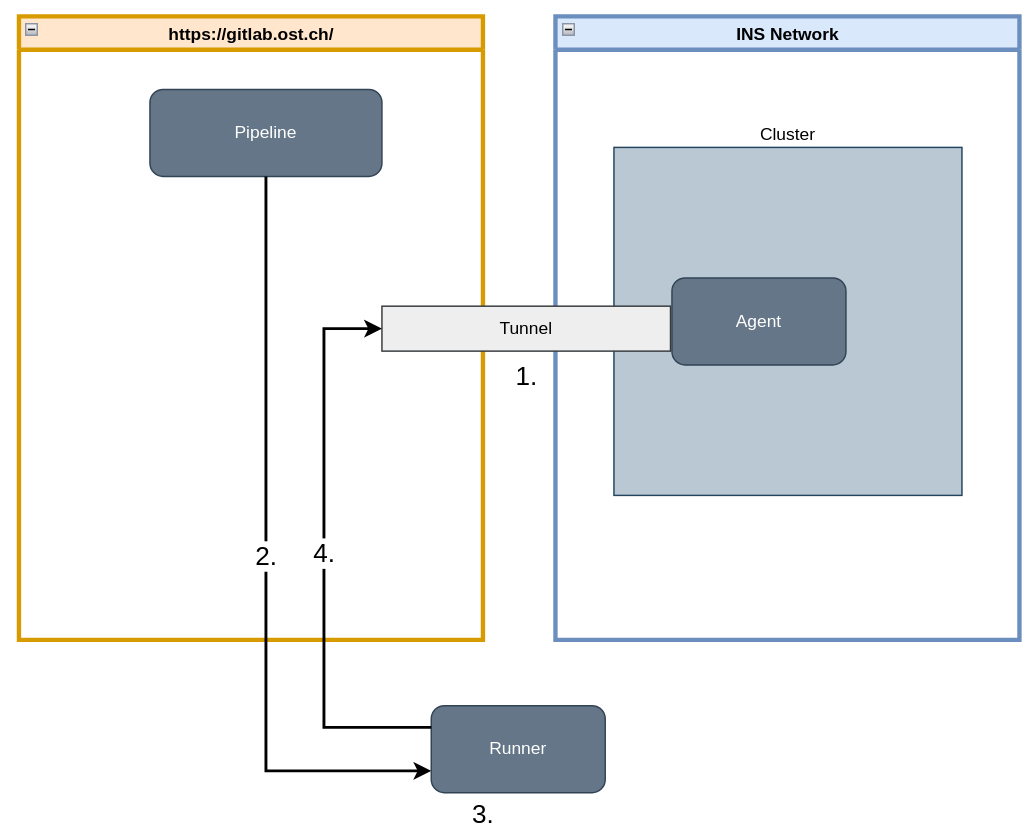
\includegraphics[height=12cm]{resources/k8s_including_in_gitlab-ost.png}
\begin{enumerate}
    \item The \textit{Agent} creates a \textit{Tunnel} from the INS network to the gitlab.ost.ch network.
    \item The \textit{Pipeline} triggers the \textit{Runner} to run the cluster commands.
    \item The \textit{Runner} starts the docker.
    \item The \textit{Runner} gets access to the \textit{tunnel endpoint} via the gitlab.ost.ch network and runs the cluster commands now at the cluster.
\end{enumerate}

\noindent The figure above shows how the Kubernetes cluster and GitLab are combined. GitLab and the cluster are in two different networks,  GitLab is placed in the OST network and the Kubernetes cluster is deployed in the INS network.

Only the \textit{Agent} inside the INS network can create the \textit{Tunnel} to the gitlab.ost.ch network. Nobody from the gitlab.ost.ch network can deploy the \textit{Tunnel} by themself.

The \textit{Runner} is independent of the location, so it does not depend on the network where you place the \textit{Runner}.